\documentclass[11pt,a4paper]{amsart}
\usepackage{setspace}
\doublespacing
\usepackage{amssymb,latexsym}
\usepackage{graphicx}
\theoremstyle{plain}
\newtheorem{theorem}{Theorem}
\newtheorem{corollary}{Corollary}
\newtheorem{lemma}{Lemma}
\newtheorem{axiom}{Axiom}
\newtheorem{proposition}{Proposition}
\usepackage{geometry}
\geometry{a4paper,left=2cm,right=2cm,top=1cm,bottom=1cm}
\theoremstyle{definition}
\newtheorem{definition}{Definition}
\usepackage{ulem} % various underlines
\usepackage[hidelinks, breaklinks]{hyperref} % to insert URL 
\usepackage{graphicx} % to insert illustration
\usepackage[mathscr]{eucal} % to express a collection of sets
\usepackage{bm} % bold font in equation environment
\usepackage{color} % color some text
\usepackage{framed} % to add a frame 
\usepackage{tikz}
\usepackage{nicematrix}
\usepackage{threeparttable}
\usepackage{tabularx, ragged2e} 
\usepackage{booktabs}
\renewcommand{\arraystretch}{1.5}
\newcommand*\circled[1]{\tikz[baseline=(char.base)]{
		\node[shape=circle,draw,inner sep=1pt] (char) {#1};}} % circled numbers
\usepackage{float}%do not auto repositioning
% $\uppercase\expandafter{\romannumeral1}$ Roman numeral
%	\begin{figure}[hbt]
	%{\centering \includegraphics[scale=0.78]{ring_algebra_semi}}
	%\caption{ring \& algebra \& semi-}\label{F:ring_algebra_semi}
	%\end{figure}
\usepackage[style=apa, eprint=false]{biblatex} %Imports biblatex package
\raggedright
\addbibresource{bib_AP_startup_project_statement.bib} %Import the bibliography file
	
\begin{document}
\title{S\lowercase{patial} D\lowercase{iffusions of the} R\lowercase{egional} T\lowercase{ourism} S\lowercase{ystem}}
\author{ X\lowercase{iaoying} (E\lowercase{den}) J\lowercase{iao}}
\date{\today}
		
\begin{abstract}
	With the increasing trend of globalization, and the competitive environment in tourist destinations, collaborative strategies have been promoted under the regional destination marketing framework either at country level or city level. Destinations are longer being considered as isolated, but instead have complex interactions with neighboring destinations from different aspects. Within each tourist destination system, tourism is an intersecting industry connecting many related industries such as accommodation, transportation, and tourist attractions, involving different sectors including tourists, destinations and communities. Thus, to evaluate the tourism system comprehensively requires a systematic approach from both macro level (i.e., destination-level) and micro level (i.e., individual-level), especially for regions with complex administrative relationships across cities such as the GBA area. This project aims to develop a systematic framework to examine the spatial diffusions of tourists in the GBA area from both macro spatial agglomeration perspective and individual tourist decision-making perspective.
\end{abstract}
		
\maketitle

\tableofcontents
\newpage

\section{Background of Research}
\subsection{Spatial Spillovers in Tourism}\hfill\par
\noindent Tourism demand modeling and forecasting, along with the rapid development and increasing importance of international tourism in the global economy, has become an important field of research for a prolonged period since the 1970s. These models and estimations are crucial for tourism demand and economic development analysis, which in turn enables effective government policy planning. \parencite{jiaoTourismForecastingReview2019}. High-quality research on tourism demand and development is also important for business practitioners and local authorities in the decision-making processes \parencite{pengMetaAnalysisInternationalTourism2015}. \textcite{songReviewResearchTourism2019} reviewed the four common types of models being used in tourism demand analysis, including time series models, econometrics models, artificial intelligence (AI) models and judgmental methods. Among those, the superior advantage of the econometric methods are the explanatory power and the potential for identifying causal relationships between economic indicators. The estimated structural econometric equations can further be used to measure variables like the price and/or income elasticity of demand, which are essential elements for economic analysis. However, it is recognized that there does not exist a model that consistently outperforms others in every circumstance in terms of modelling and forecasting tourism demand \parencite{liRecentDevelopmentsEconometric2005, wuNewDevelopmentsTourism2017}. 

\noindent Although sophisticated econometric methods have been implemented for the precision of estimation and prediction, most of existing studies treat destinations as independent units. However, as any economic activity, the tourism demand of a destination is highly correlated and interdependent with that of the neighbors \parencite{longPoolingTourismDemand2019}. Tourism development in one destination affects not only the economic outcomes within the territory, but also produces a spillover effect on other regions if they are close from a geographic or economic perspective (or both) \parencite{liTourismRegionalIncome2016}. The theoretical foundation of the spillover effects in tourism could be attributed to the cluster theory \parencite{kimVisitorFlowSpillover2022}. \textcite{porterCompetition2008} defines a \textit{cluster} as a geographically proximate group of interconnected companies and associated institutions in a particular field, linked by commonalities and complements. The agglomeration of firms could be beneficial through the multiplier and positive externality for the local economy, as illustrated by \textcite{berniniConventionIndustryDestination2009} in the study on the convention industry in Italy. Since the geographical proximity, potential consumers can reduce their searching costs significantly. The accumulation of reputation will also further attract customers to the location \parencite{kuahClusterTheoryPractice2002}. On the supply side, the benefits include knowledge spillovers, infrastructure benefits and the ready availability of skilled labor in the area \parencite{kuahClusterTheoryPractice2002}. The spatial spillover effect follows naturally if we think different tourism destinations in a region as firms within the same industry. For example, \textcite{michaelTourismMicroClusters2003} highlights the clustering effects driven by the development of tourism  on economic opportunity in small communities. The increase in tourist arrivals (and hence, the tourism revenues) echoes the investment in infrastructure and human capital in a reciprocally beneficial way. Meanwhile, the nearby destinations may benefit from the demonstration (and learning) effect, the labor movement and the competition effect from that place \parencite{longPoolingTourismDemand2019}. The synthesis of tourism destinations also happens through other mechanisms, for example, joint promotion activities, accidents (e.g., terrorist attacks) and multi-destination travel patterns \parencite{yangSpatialEconometricApproach2012}. However, traditional econometrics assumes the tourism demand is endogenously determined within the region and therefore neglects spillover effects from others in the economic system. This problem could be substantial, especially for destinations with similar cultural backgrounds (e.g., cities in China). The confounding effects of underlying spatial structure lead to potentially biased estimators for the estimands of interest. Panel data could alleviate this problem as it takes into account both the time and space dimensions for the estimation. And these data can be used to estimate the dependence of the destinations in the system, as well as the spatial heterogeneity of them. 

\noindent Researchers have begun to apply spatial econometric methods to model and estimate tourism demand and development \parencite{dengModellingAustralianDomestic2011, marrocuDifferentTouristsDifferent2013}, as well as the spatial spillover effect of tourism growth \parencite{yangSpatialEffectsRegional2014, maTourismSpatialSpillover2015}. Spatial econometrics has also been used in industrial-level research. \textcite{adamPerceivedSpatialAgglomeration2014} evaluated the perceived spatial agglomeration effects on hotel location choice. \textcite{gunterModelingAirbnbDemand2020} used a spatial Durbin model (SDM) to estimate the spillover effect of Airbnb demand in New York City. As for the tourism resorts, \textcite{kimVisitorFlowSpillover2022} explored the visitor flow spillover effects in London on attraction using a spatial econometric model. The interdependence of tourism activities between cities in China has also been confirmed. \textcite{yangSpatialEffectsRegional2014} found a significant spatial correlation between the regional tourism developments in China. \textcite{liuEffectsTourismDevelopment2022} constructed both static and dynamic spatial Durbin models to explore the effects of tourism development on economic growth. These studies show the great power of spatial econometrics models on tourism economics research. 

\noindent Based on the existing literature, this project identifies the limitations of current research and the unique challenges for spatial tourism econometrics research in the case of the Greater Bay Area. 
\begin{enumerate}
	\item The spillover effects are assumed to be homogeneous in traditional spatial models. This is an unrealistic assumption, and incapable of capturing the dynamics in the time dimension for complex tourism systems like the GBA.
	\item The homogeneity assumption is also insufficient in terms of modeling the asymmetry of spillover effects across the cities in the GBA, which is expected to be significant due to the different development stages of these regions.  
	\item The geographic and political relationships are complicated in the GBA. However, a single spatial weighting matrix is limited in terms of explanatory power. Meanwhile, a single-level spatial model cannot capture the effects from higher levels (e.g., provincial and special administrative region) variables. 
\end{enumerate}

\noindent This project develops cutting-edge spatial econometrics models to address these limitations. The specific model settings will be further discussed in the methodology section. 

\subsection{Tourism Destination Choice}\hfill\par
\noindent As tourism destinations are complicated with different components, one of the most important component is the tourists. Although efforts has been made to model tourism demand by using a wide range of econometric methods or artificial intelligence methods using aggregated normally at the destination level, as \textcite{songReviewResearchTourism2019} has suggested, the use of disaggregated data is one of the major research directions to avoid misspecification of individual decision making \parencite{masieroUnderstandingHotelLocation2019}. The focus on the decision-making process to select destination provides a platform to model tourism demand from individual tourist level instead of an aggregated level \parencite{baltasEconometricModelsDiscrete2007}. 

\noindent Research on tourist destination choice relies on the random utility theory \parencite{huybersDomesticTourismDestination2003}, which states that when tourists select destinations, they tend to compare the overall utility of each possible destination choice set and choose the one with the highest utility based on the rank-order utility maximization rationale \parencite{yangMODELINGSEQUENTIALTOURIST2013}. Although utility of each choice set is unobservable, the final choices can be observed and used to deduct the rank order of each choice set. Many tourist studies have analyzed the attributes that affect utility of each destination and further affect destination choice, such as regular attributes of a destination including travel resources, service quality, and accessibility, travel costs and quality of service and overall satisfaction \parencite{masieroModelingReferenceExperience2018}. Apart from those widely analysed attributes, \textcite{masieroModelingReferenceExperience2018} has considered individual tourists’ typical destination by integrating a focal function into destination attribute based on the prospect theory \parencite{kahnemanProspectTheoryAnalysis1979, tverskyAdvancesProspectTheory1992} stating that individuals evaluate outcome based on a reference point. In tourist destination choice model, past experience of destination choice (i.e., typical destination) is considered as a reference point when making choice decisions. 

\noindent Another important direction of destination choice decision research is the interrelationship of destination choices in a single trip. This corresponds to the spatial agglomeration theory that mentioned above, stating that destinations are not isolated given the existence of spatial spillovers being proven in many empirical studies \parencite{yangSpatialEconometricApproach2012}. \textcite{wuTouristMultiDestinationChoice2012} developed a new destination choice model based on the concept of future dependence (i.e., destination that will be visited in the later) using a mother logit model and results reviewed that travel time, diversity of destination and variety seeking significantly affect multi-destination choice behaviour. \textcite{yangMODELINGSEQUENTIALTOURIST2013} analysed multi-destination travel patterns from a subsequent decision-making perspective by partitioning the decision process into multiple stages with determinants identified by nested logit model at each stage. Results show that apart from destination and individual factors, spatial structures of the destinations also significant influence sequential choices. 

\noindent Following the above direction, this project will take into account the interrelationship of destination choices in the GBA area, by considering geographic factors and social interaction factors given the complex relationship in the GBA cities when simulating the individual tourist decision making utility function. This interrelationship corresponds to the spatial spillovers caused by world-of-mouth (social interactions) and multi-destination travel patterns (accessibility and geographic factors). However, the two factors are not empirically tested in the macro spatiotemporal econometric model. Thus one major contribution of this study is to explain this spatial spillovers of tourism demand from individual destination selection procedure from the demand perspective of spillover. 

\subsection{ABM in Tourism}\hfill\par
\noindent Modelling individual choice selection behaviour reflects individual decision making procedure and individual heterogeneity, whereas understanding the whole complex tourism system requires to account for interactions of different components in the system. To model complex phenomena of social relationship and behaviours, agent-based modelling has been frequently used in social science research and in tourism research due to the complex nature of the tourism system \parencite{boavida-portugalWhereVacationAgentbased2017}. ABM modelling framework has been employed to analyse different aspects in tourism, such as tourist decision making,  tourist flow management and cultural tourism management. In tourist decision making analysis, studies model at the individual level first, to incorporate individual heterogeneity and diversity in attributes and behaviors interacting in the system by adopting a bottom-up approach \parencite{macalTutorialAgentbasedModelling2010}.

\noindent \textcite{boavida-portugalWhereVacationAgentbased2017} developed an ABM modelling framework to understand where and why tourist decide to vacation based on a theoretical proof-of-concept perspective with tourists and destinations being the two types of agents identified in the study. Within the ABM system, tourists are affected with social influence and individual level influence when making decisions to travel to one of the five destinations with attraction list provided and motivations assumed beforehand which are matched with destination attractiveness. The relationships between factors that determines the decision procedures are parameterized in the ABM system firstly based on theoretical foundation, and the parameters are then calibrated and validated using real data. Two experimental scenarios has been conducted and results show that destination awareness and individual preferences shapes destination choices. \textcite{liAgentBasedModelingSpatial2021} develops a simulated framework of visitor flows that incorporates the interactions between visitor agents (i.e., attributes and decision making rules) and environment (i.e., destination and attraction). In the study, the agents were classified into three categories based on decision patterns, namely global optimizers, sequential optimizers and radial optimizers, and the utility maximization decision-making rules has been identified for each agent type for simulation. To account for the magnitude of spillover, the frequency of cross-boundary travel has been measured to represent spillover effects generate in the simulated system. The results is further validated with exploratory spatial data analysis and results show that western cities have lower level of spillover effects than the eastern cities. \textcite{qiuAgentbasedModelingSpatial2016} has also investigated the spatial tourist diffusions process of tourism system in Sichuan by integrating micro-level tourist behaviors with a macro-level tourist flow structure in a regional tourist spot system. Both tourist agents and tourist spot’s manager agent and the environment are incorporated within the ABM system in which tourist spot-selection and route scheduling behaviors and tourist-spot management behaviors are investigated simultaneously. Tourist flows (i.e., spatial diffusions) of tourist spots have been simulated in the Sichuan area.

\section{Aims and Objectives}
The aim of this project is to unravel the complexity of spatial diffusions of tourism system in the GBA area from multiple perspectives. The detailed objectives are as follows:
\begin{enumerate}
	\item To model the spatial interactions and transmission mechanism of tourism development in the cities in the GBA area by using a series of cutting-edge spatiotemporal econometric models with the use of aggregated macro-level data from official statistics.
	\item To model the tourist destination choice decision-making procedure to verify the demand-side factors causing spatial spillovers across destinations (i.e., multi-destination travel patterns and world-of-mouth effect) from experimental design using different destination sets in the GBA area. 
	\item To simulate tourists’ visiting patterns in the GBA area by using agent-based modelling and conduct scenario testing to aggregate individual tourist behaviors into macro-level influence on the whole GBA tourism system.
	\item To compare the findings from official statistics and aggregated findings derived from individual tourist decision making process to verify the spatial diffusion mechanism of the GBA tourism system.
\end{enumerate}

\section{Research Plan}\hfill\par 
\noindent As mentioned above, this project will develop an integrative and comprehensive framework in muti-stages of measuring spatial diffusions of tourism demand and tourist flows across the cities in the GBA area from both macro perspective (destination-level), micro perspective (individual-level) and the combined perspective. At the first stage, this project will examine the spatial diffusion mechanism of tourist flows in the GBA area using aggregated tourism and economic statistics data, by taking into account spatial interactions, hierarchical and multilevel relationship across cities and regional tourism development differences. At the second stage, the demand side factors of spatial spillovers including multi-desitnation travel patterns and the world-of-mouth effect will be empirically tested at the tourist level by using an experimental design including multiple destination set in the GBA area. Finally the findings from the macro study and the micro study will be cross validated in the ABM framework to simulate spatial diffusions of tourist flows in the GBA area.

\section{Methodology}
\subsection{Hierarchical Spatiotemporal Model}\hfill\par 
\noindent Given the particularity of the administrative and geographic division of the GBA, the single spatial weighting matrix in traditional spatial econometrics models are inadequate in terms of the relationships between cities in the area and those near the border. Therefore, this project decomposes the spatial spillover effects inside and outside the region and across them by using multiple weighting matrices. As an example, in this project, the higher-order dynamic spatial Durbin model (SDM) could be written as 
\[	y_{it} = \rho y_{it-1} + \lambda_{1} \sum_{j \ne i}^{N}w_{ij}^{\text{non-GBA}}y_{jt} + \lambda_{2}\sum_{j \ne i}^{N}w_{ij}^{\text{GBA}} y_{jt} + \lambda_{3}\sum_{j \ne i}^{N}w_{ij}^{\text{Cross}} y_{jt}  + \beta x_{it} + \theta \sum_{j \ne i}^{N}w_{ij}x_{jt} + \mu_{i} + \epsilon_{it}.	\]
In this equation, $y_{it}$ is the tourism income of city $i$ in period $t$. $\lambda_{1}$ is the coefficient on the weighted average of the tourism income of cities \textit{outside} the GBA, $\lambda_{2}$ is the coefficient on the weighted average of the tourism income of cities \textit{inside} the GBA, and $\lambda_{3}$ is the coefficient on the weighted average of the tourism income of cities \textit{across} the sub-systems (i.e., the GBA and non-GBA areas). $\beta$ and $\theta$ give information about the effects of $x$ on the dependent variable $y$. These will be the estimands of our main interest. $w_{ij}^{\text{GBA}}$ measures the strength of dependence (defined by distance or commute time) between city $i$ and $j$ \textit{inside the GBA}. If city $i$ or $j$ is not in the GBA, then $w_{ij}^{\text{GBA}}$ is defined to be $0$. $w_{ij}^{\text{non-GBA}}$ and $w_{ij}^{\text{Cross}}$ are defined similarly, with $w_{ij}^{\text{non-GBA}} = 0$ if city $i$ or $j$ (or both) is in the GBA, and  $w_{ij}^{\text{Cross}} \ne 0$ only if $i$ and $j$ are in different sub-systems. $x_{it}$ is a vector of control variables, $\mu_{i}$ is a city fixed effect and $\epsilon_{it}$ is the error term. 

We use Two-stage least-squares regression (2SLS) for estimation. The estimated $\widehat{\lambda}_{1}$,  $\widehat{\lambda}_{2}$ and  $\widehat{\lambda}_{3}$ measures the interdependence and synthesis effects of the cities inside, outside and across the GBA, respectively. Different from the traditional econometric models, we cannot take $\widehat{\beta}$ simply as the effect of $x$ on the panel system and the sub-systems. Instead, we average over the diagonal terms in the resulting Jacobian matrix to get the direct effect of $x$ on tourism revenue. The indirect effects are measured by the average of the off-diagonal elements. Moreover, these indirect effects can further be decomposed into sub-system and cross-system effects. The estimation of these parameters helps us understand the mechanism of tourism development in the GBA and the country.
		
\subsection{Spatial Two-Regime Model}\hfill\par 
\noindent After basic modeling setting and calibration, this project introduces two-regime spatial econometric models to further formalize the spillover effects in time and space dimensions. In the time dimension, we investigate the effect of the establishment of the GBA on tourism development in terms of the spillover and agglomeration effects. We choose March 2017 (the first time when the GBA plan appears in the government report) as a cutoff point for our analysis. In order to overcome the potential omitted variable bias and the shortcomings of the two-regime spatial lag model (which does not control for the $WX$ variables), \textcite{elhorstEvidencePoliticalYardstick2009} suggests including the spatial lags of both the dependent and independent variables for the analysis. We also include the space and time fixed effects to correct for the time-persistent and spatial-persistent variables in the error terms. The structural equation of our two-regime spatial Durbin model could be written as  \parencite{wangStrategicInteractionIndustrial2020}
\[	y_{it} = \delta_{1}d_{it}\sum_{j = 1}^{N}w_{ij}y_{jt} + \delta_{2}(1-d_{it})\sum_{j = 1}^{N}w_{ij}y_{jt} + \beta x_{it} + \theta \sum_{j = 1}^{N}w_{ij}x_{jt} + \mu_{i} + \lambda_{t} + \alpha + \epsilon_{it}.	\]
In this equation, $y_{it}$ is the tourism development indicator of city $i$ at time $t$. In this project, we use tourist arrivals and tourism revenues as the indicators. $w_{ij}$ measures the relationship of city $i$ and $j$, and these give us a $N$-by-$N$ weighting matrix $W$. There are various ways to define $w_{ij}$, and we will provide more details in the later sections. $x_{it}$ is a vector of independent variables affecting tourism development, such as income and price levels. Although we include all cities in a single panel, the heterogeneity of each city cannot be neglected. $\mu_{i}$ represents the city fixed effect that controls for all space-specific, time-invariant variables. And $\lambda_{t}$ represents the time-period fixed effects which control for all time-specific, spatial-invariant variables. $\sum_{j = 1}^{N}w_{ij}y_{jt}$ is the spatial lag of the dependent variable, and its coefficients $\delta_{1}$ and $\delta_{2}$ capture the spatial spillover effect in different contexts (more on this later). Similarly, $\sum_{j = 1}^{N}w_{ij}x_{jt} $ is the spatial lag of the independent variables, and $\theta$ represents the spillover effect of the socio-economic conditions of other cities on the tourism development of $i$. 

\noindent We define the dummy variable $d_{it} \in \{0, 1\}$ in two different approaches. First, we let $d_{it} = 1$ if city $i$ is in the GBA and $t$ is after 2017, and $d_{it} = 0$ otherwise. With this definition, we can evaluate the effect of the establishment of the GBA on tourism development for cities in the area. $(1-d_{it})\sum_{j = 1}^{N}w_{ij}y_{jt}$ and $d_{it}\sum_{j = 1}^{N}w_{ij}y_{jt}$  represent the spatial interdependence of the tourism development in city $i$ with other cities before (i.e., the first regime) and after (i.e., the second regime) the establishment of the GBA, respectively. The coefficients $\delta_{1}$ and $\delta_{2}$ suggest the level of spatial interdependence. If $\delta_{1}$ is greater than $\delta_{2}$ both statistically and substantively, we may conclude that the establishment of the GBA has a positive effect on the tourism destinations agglomeration effect.

\noindent  We can also define $d_{it} \in \{0, 1\}$ as follows. Let 
\[	d_{it} = \begin{cases}
	1, &\text{if $y_{it} > \sum_{j = 1}^{N}y_{jt}$;}\\
	0, &\text{otherwise.}
\end{cases}	\]
In words, if the tourism development level of city $i$ is higher than other cities at period $t$, then we set $d_{it} = 1$. If city $i$ is a ``less-developed/weak'' city, then $d_{it} = 0$. Now, we can investigate the spatial spillover effects that account for the heterogeneity of development stages of different cities. According to the significance level and signs of $\delta_{1}$ and $\delta_{2}$, we can further identify different forms of the spillover of the cities in the GBA. We list these nine forms in table (\ref{tb:9cptb}). 

\begin{singlespace}
	\begin{table}[H] 
		\caption{Nine forms of the spillover effects.}\label{tb:9cptb}
		\begin{threeparttable}
			\begin{center}
				\begin{NiceTabular*}{\linewidth}{@{\extracolsep{\fill}}cccc}
					\hline
					& $\delta_{2} < 0$ & $\delta_{2}$~\text{insignificant}  & $\delta_{2} > 0$ \\ 		
					\hline 
					&&&\\
					\parbox{2cm}{$\delta_{1} < 0$} & \parbox{4cm}{completely suppressed \\by the development of neighbors} & \parbox{4cm}{suppressed by the development of weak neighbors} &  \parbox{4cm}{suppressed by the development of weak neighbors, reinforced by the development of strong neighbors} \\
					&&&\\
					\parbox{2cm}{$\delta_{1} ~\text{insignificant}$} & \parbox{4cm}{suppressed by the development of strong neighbors}	 &   \parbox{4cm}{independent \\development}  &  \parbox{4cm}{reinforced by the development of strong neighbors}   \\
					&&&\\
					\parbox{2cm}{$\delta_{1} > 0$}	&  \parbox{4cm}{reinforced by the development of weak neighbors, suppressed by the development of strong neighbors}	&  \parbox{4cm}{reinforced by the development of weak neighbors}	  & \parbox{4cm}{completely reinforced \\ by the development of neighbors}	 \\
					&&&\\
					\hline
				\end{NiceTabular*}
			\end{center}
			\begin{tablenotes}
				\item Sources: \textcite{diaoSpatialSpilloverEffect2021} and the authors’ own compilation.
			\end{tablenotes}
		\end{threeparttable}
	\end{table}
\end{singlespace}

\subsection{Experimental Design}\hfill\par 
\noindent To test the individual decision making process in the GBA destination specifically, this project will employ an experimental design method to analyse the interrelationship of destination choice. Basically destinations will be included in multiple sets to reflect how individual-level destination choices are influencing each other. The experiment scenarios and destination choice set will be developed carefully to design a series of GBA-applicable scenarios and attribute dimensions instead of including only generic attributes. A thorough desk research of the GBA area and GBA-related tourism literature will be conducted first, followed by using the Delphi method to conduct in-depth interviews with academic professionals to evaluate the scenario settings. Currently the destination attribute dimensions will follow \textcite{masieroModelingReferenceExperience2018} to include cultural attractions, natural attractions, outdoor recreational attractions, entertainment attractions, hospitality services, food and dining services, transportation services, and price. Other attributes related to destination image will be incorporated as well following \textcite{kirillovaDevelopingCoopetitiveDestination2020}, including affective image, cognitive image and destination quality in the 11 cities in the GBA area. 

\noindent The experimental design will be conducted through distributing survey to tourists in China. The tourists will be divided into two groups, including GBA tourists and Non-GBA tourists. To model the destination selection rationale, a mixed multinomial logit (MMNL) will be employed for estimation. Different from previous literature, the utility function in this study will incorporate both social interactions and spillovers from other GBA destinations. The utility of selecting destination $p$ for individual $i$ with the consideration of social spillover and destination spilllover can be specified as 

\[	U_{pi} = V_{pi}(X_{pk} \mid \beta_{ki}) + \sum_{j = 1}^{N} w_{ij}V_{pm}(X_{pm}\mid \lambda_{kj}) + \sum_{q = 1}^{M}w_{pq}V_{qi}(X_{qi}\mid\gamma_{ki}) + \epsilon_{ij}.	\]

\noindent Here $V_{pi}$ is the standard value function of destination $p$’s attributes. Social interactions is reflected in $ \sum_{j = 1}^{N} w_{ij}V_{pm}(X_{pm}\mid \lambda_{kj})$, where $w_{ij}$ represents the social relationship between individual $i$ and individual $j$. $\lambda_{kj}$ is the estimated level of effects from social interaction in shaping destination choices. Destination-level spillovers reflecting multi-destination travel patterns is denoted by $\sum_{q = 1}^{M}w_{pq}V_{qi}(X_{qi}\mid\gamma_{ki})$, where several specifications of $w_{pq}$ will be empirically tested, capturing administrative relations, geographical distance and transportation time between each pair of cities in the GBA area. $\gamma_{ki}$ is the estimated level of effects from multi-destination travel patterns.

\subsection{Agent-Based Modeling (ABM)}\hfill\par 
\noindent Similar to the simulated framework proposed by \textcite{liAgentBasedModelingSpatial2021}, the basic ABM framework in this study will also include three agents, namely visitor agents (proxy of individual tourists), environment (proxy of destination) and their interactions (proxy of destination choice decision-making process). Visitor agents are interrelated as well, by capturing the social interaction effects in pre-categorised social groups (i.e., latent class identified in the previous stage of this project). Environment (i.e., cities in the GBA area) are interrelated as well in the simulated system, which is captured by the administrative relationship, geographical distance and transportation convenience across cities in the GBA area. The procedures of ABM simulation is as follows in Figure (\ref{F:meth_stul_ABM}).

\begin{figure}[hbt]
	{\centering 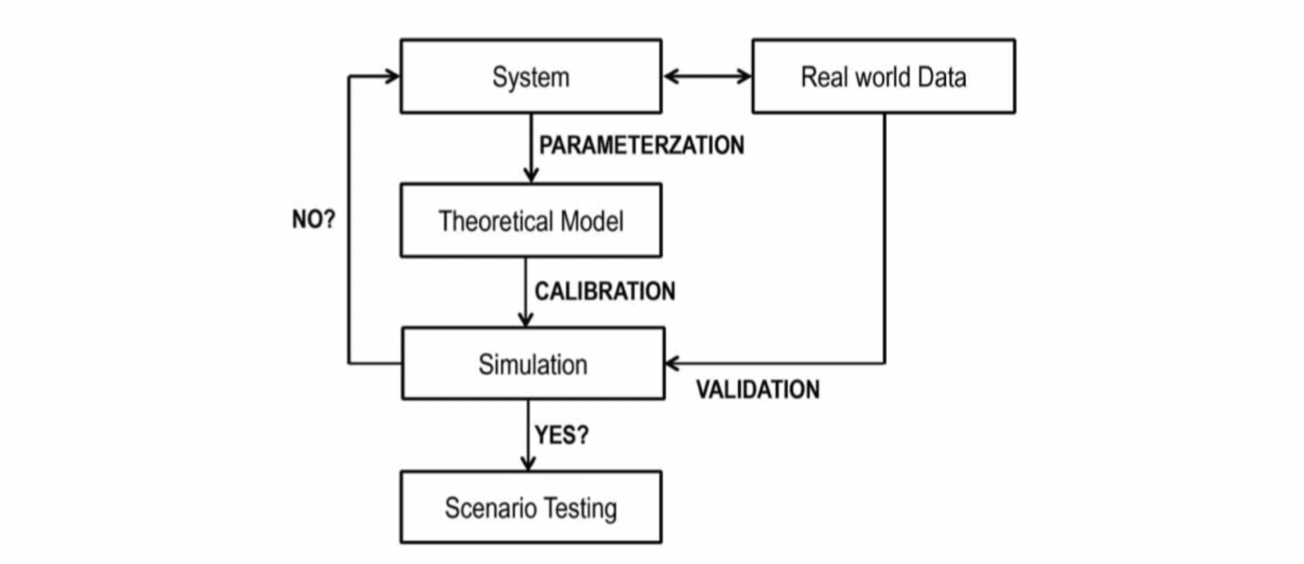
\includegraphics[scale=0.58]{meth_stul_ABM}}
	\caption{Methodological Structure of the ABM}\label{F:meth_stul_ABM}
\end{figure}

\noindent The parameterization will be based on tourist decision making rules derived from theoretical framework, previous literature and the findings from the previous experimental design research. The theoretical model will be further calibrated using real world data for validation and if the individual level tourist flows can reflect aggregated level real word situation, then the system will be further employed for scenario testing. Another important setup of  the ABM system is the categorization of tourist types. Different types of tourist will have different decision making rules. The classifications will be determined based on the findings in the previous stages and in-depth interviews with practical professionals in tourism bureaus. 

\subsection{Data}\hfill\par 
\noindent Secondary data collection will be conducted in the first stage for the macro study on destination spatial diffusions. Data on city-level tourism statistics, economic and social statistics will be collected in official statistics such as China Statistic Yearbook at city level in mainland China, Hong Kong Tourism Board (HKTB) and the Statistics and Census office (DSEC) in Macau.
Primary data collection will be conducted in the second and third stage of the project. Surveys including the experimental design will be distributed to GBA and Non-GBA tourists and qualitative in-depth interviews will also be conducted in multiple stages to ensure the quality of the experiments and the scenario settings.

\section{Project Outcomes and Deliverables}\hfill\par
\noindent The major outcome of this project is the development of a comprehensive and integrative macro-micro framework to examine the spatial diffusions of the tourism system in the GBA area. This multi-stage project includes several studies, which will be translated into two submissions in top-tier journals such as Annals of Tourism Research and Journal of Travel Research. Preliminary findings of this research will at the International Association of Tourism Economics (IATE) conference held in 2023.

\noindent Beyond academia, practically this project will generate some implications for destinations in the GBA area. The final findings of this project will be written into a white report to distribute to the tourism industry through social media of the investigators, School channels and the annual IMPACT conference held in SHTM polyU to generate more practical contributions to the tourism industry.  

\vspace{20pt}
\section{Budget and Budget Justification}
\begin{singlespace}
	\begin{table}[H] 
			\begin{center}
				\begin{NiceTabular*}{\linewidth}{@{\extracolsep{\fill}}ll}
				\toprule
				Items & Amount\\
				\midrule
				\textbf{Staffing - Postdoctoral fellow} & \\
				\phantom{ZZ} Salary (12 months) & 30,000 $\times$ 12 months\\
				\phantom{ZZ} MPF & 1,500 $\times$ 12 months\\
				\textbf{Total staffing} & HKD 378,000 \\
				\textbf{General expenses} & \\
				\phantom{ZZ} Data collection & 44,000 \\
				\phantom{ZZ} Research visits to the UK & 31,000 \\
				\phantom{ZZ} Inviting Co-I to visit & 31,000 \\
				\phantom{ZZ} Conference & 16,000 \\
				\textbf{Total General} & HKD 122,000 \\
				\textbf{Total} & HKD 500,000 \\
				\bottomrule
				\end{NiceTabular*}
			\end{center}
	\end{table}
\end{singlespace}
\newpage

\section{Plan of Collaboration}
$\bullet$ PI: Dr Eden Jiao

\noindent Dr Eden Jiao will be responsible for most of the work, including developing research plans, designing theoretical framework, collecting data, hiring and supervising research personnel, constructing and implementing model for data analysis, writing journal manuscripts, disseminating research findings and ensuring the overall quality of the project is maintained. 
\vspace{3pt}

$\bullet$ Co-I: Dr Richard Qiu

\noindent Dr Richard Qiu will contribute to this project mainly in data collection and data analysis, as well as writing journal manuscripts and disseminating research findings.
\vspace{3pt}

$\bullet$ Co-I: Prof Gang Li

\noindent Prof Gang Li will contribute to this project mainly in developing research plans, supervising research personnel, reviewing and editing journal manuscripts and ensuring the overall quality of the project is maintained. 

\section{Contributions of the Project to Teaching and Learning}
\noindent This project will generate several contributions to Teaching and Learning beyond academia. To begin with, this project will use a wide range of different methods. Those systematic approaches can be taught to post-graduate level students with examples of data sample used in this project for hands-on practice. The methods and findings can be introduced in Research Methods, Tourism Economics and PhD statistics modules at different levels. Methodological workshops can be held as well to introduce the use of the family of spatiotemporal econometric methods and the ABM methods to explore the applicability of those methods in different disciplines and promote more collaborations. Practical implications related to destination image, destination management and marketing can also be taught to students to have an understanding of tourism destination management and how real-life tourism industry can be affected and benefited by academic research.

\section{Significance and Value of the Project to SHTM}
\noindent This project can also bring value to SHTM. Firstly, as mentioned above, the methodological framework of the widely applicable spatial econometric methods and ABM methods can broaden our post-graduate students’ horizon to explore more possibility in their own research and promote more collaborations with colleagues within SHTM. Secondly, this project will be internationally collaborated with University of Surrey. Academic visits between the two universities will be facilitated during the project periods to further promote more international collaborations in the two schools. Moreover, as the topic is closely related to the real tourism industry in the GBA area, practically the project findings will be distributed through media channels to the tourism and hospitality industry to generate greater practical impact. This project will also be used as a foundation of a series studies of related to ABM simulations with tourists, employees, destinations and hospitality organizations as agents across different levels and future external grant applications. 

\printbibliography %Prints bibliography
		
\end{document}
